\documentclass[a4paper,11pt,titlepage]{article}

\usepackage[utf8]{inputenc} 
\usepackage[T1]{fontenc}      
\usepackage[francais]{babel} 
\usepackage[top=4cm, bottom=4cm, left=4cm, right=4cm]{geometry}
\usepackage{graphicx}

\title{Le numérique dans l'accomplissement des SDGs}
\author{Djavan Sergent}

\begin{document}
	\maketitle
	\tableofcontents
	\listoffigures
	\listoftables
	
	\section*{Abstract}
		abstract
	
	\section{Introduction}
		En 2000, les Nations-Unies lancent le programme des Millenim Developpment Goals (MDGs) qui s'étend jusq'en 2015. Il s'agit d'un ensemble d'objectifs internationaux parmi lesquels on peut notamment citer l'éradication de l'extrême pauvreté et de la faim, combattre la mortalité infantile ou encore apporter une éducation à toutes et tous. Les 191 états membres des Nations-Unies ainsi que 22 organisations internationnales se sont engagées à participer activement à la réalisation de ces objectifs.
		\begin{figure}
			\begin{center}
				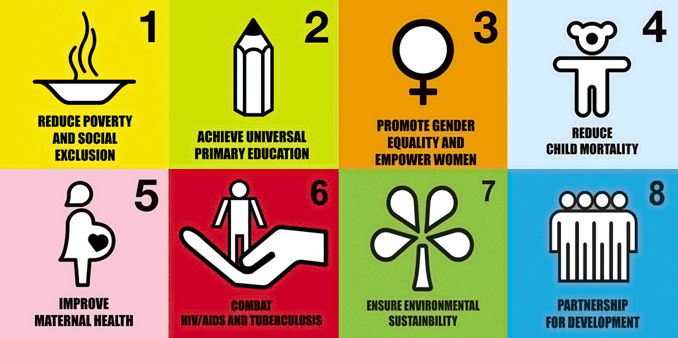
\includegraphics[width=200pt]{mdgs-full.png}
			\end{center}
			\caption{Représentation des MDGs}
		\end{figure}

		La situation en 2015 était que beaucoup d'efforts ont été investis, mais les progrès sont encore très inégaux. Les différents pays membres des Nations-Unies ainsi que des organisations civiles se sont donc intéressées à l'agenda post-2015, c'est à dire aux objectifs futurs. Les Sustainable Developpment Goals (SDGs) ont étés acceptés comme relève des MDGs. Ceux-ci comportent 17 buts, chacuns subdivisé en objectifs. Les SDGs totalisent 169 objectifs possédant chacuns leurs propres indicateurs.
		\begin{figure}
			\begin{center}
				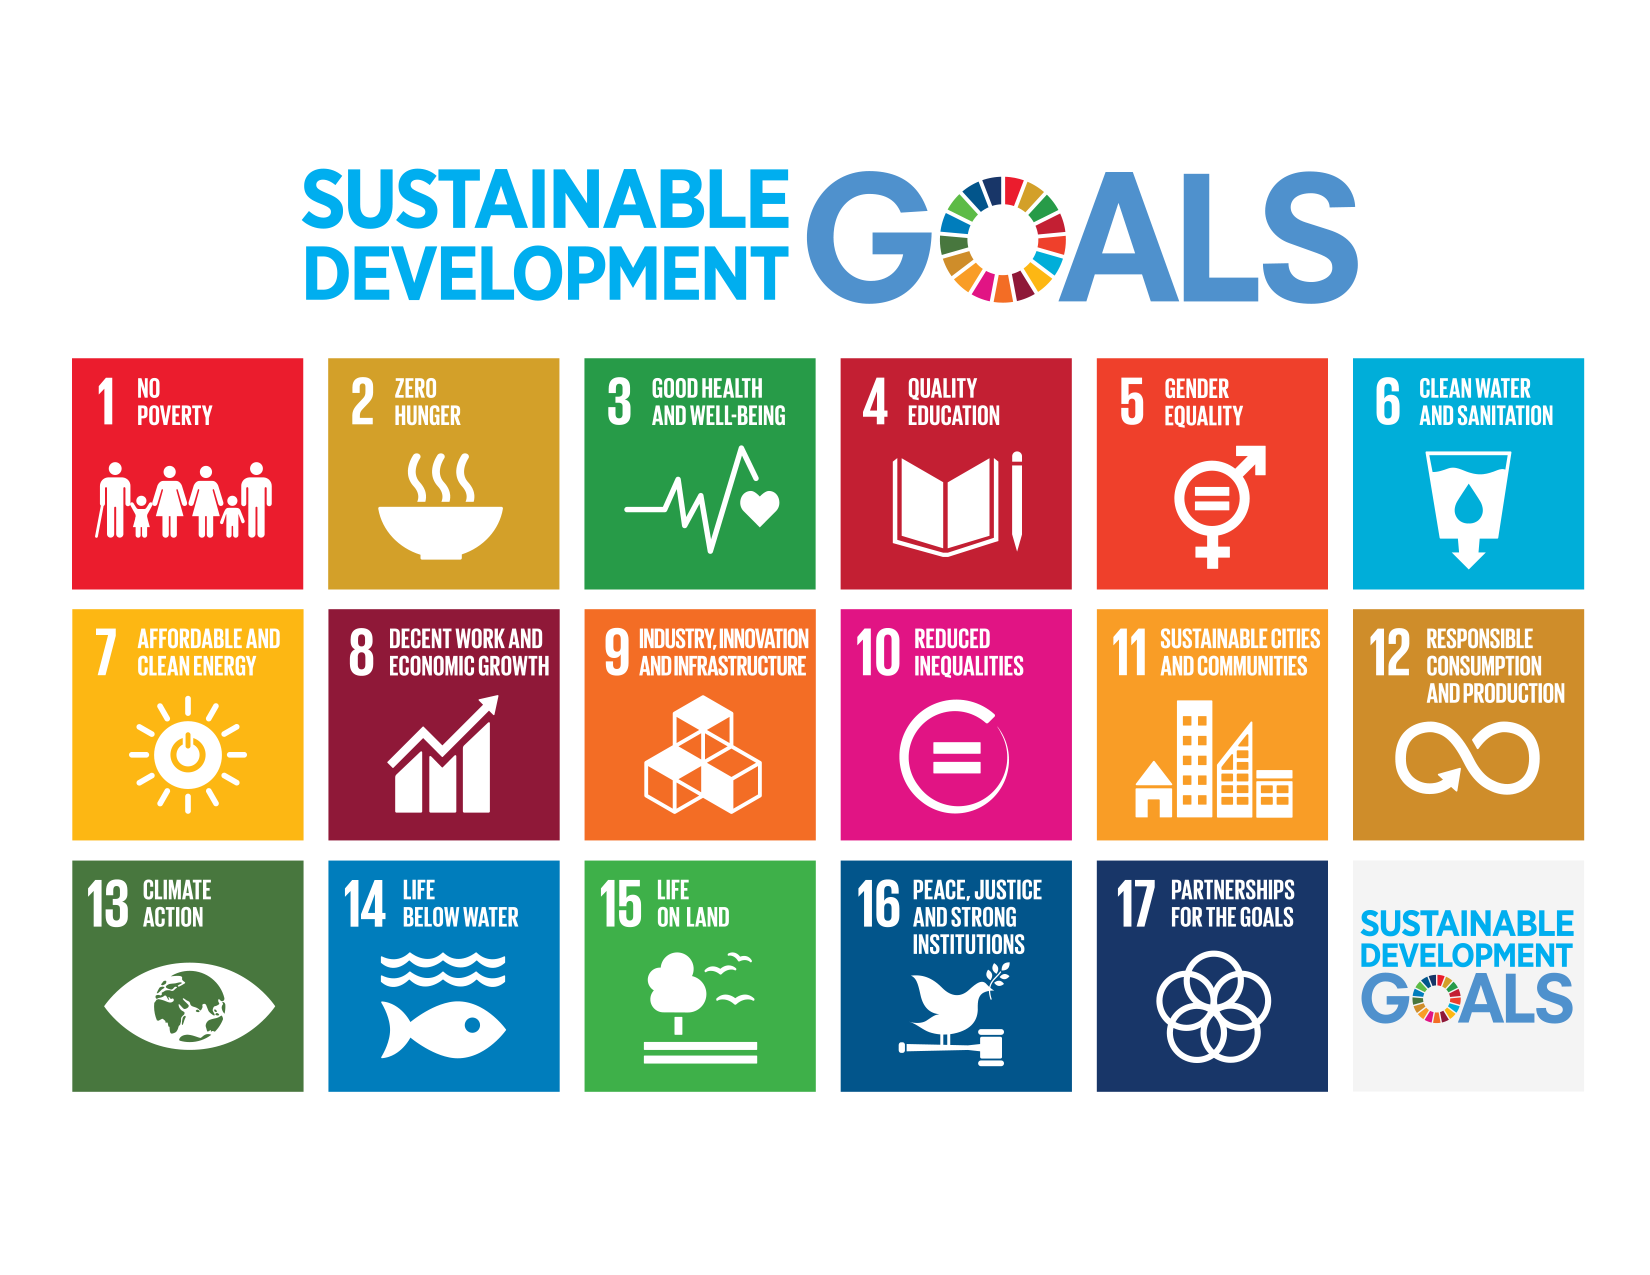
\includegraphics[width=200pt]{sdgs.jpg}
			\end{center}
			\caption{Représentation des SDGs}
		\end{figure}
		
		Nous analysons dans cet article le rôle du numérique dans la réalisation et le monitoring de certains de ces objectifs, particulièrement du point de vue de la participation citoyenne.
		 
		\subsection{Sustainable Developpment Goals}
			\subsubsection{Objectifs}
				Nous nous intéressons, dans le cadre de cet article, aux objectifs décrits ci-dessous. Il est cependant important de noter que les objectifs sont intrinséquement liés entre eux et s'influencent mutuellement. Par exemple, en formant des citoyens à l'utilisation de matériel de mesure de qualité de l'eau on va agir non seulement sur la capacité à, entre autre, détecter la pollution mais également sur l'éducation.
				\begin{description}
					\item[ 3 - Good-Health and Well-Being :] Cet objectif se concentre sur les aspects qui	concernent la santé, et en particulier la mortalité maternelle, natale et infantile, les maladies infectieuses, les morts prématurées, la polution de l'air, la sécurité et la mise en place de systèmes de soins et de financement.
					\item[ 6 - Clean water and sanitation :] Un accès universel à l'eau et aux installations sanitaires est essentiel pour la santé humaine, la prospérité économique et la préservation de l'environnement.
					\item[13 - Climate Action :] En 2016 s'est établi un nouveau record de température. Le réchauffement climatique peut provoquer créer, accélerer ou amplifier les aléas	naturels tels que sécheresse, inondations, cyclones ou périodes de grande chaleur. L'objectif a pour but d'agir sur les causes du réchauffement climatique.
					\item[14 - Life below water :] L'acidification des océans, la surpêche ou encore la pollution marine ont un impact important sur la protection des océans. Leur dégradation provoque des effets sur certaines espèces marines mais également sur la biodiversité et le fonctionnement des écosystèmes.
					\item[15 - Life on land :] D'importants efforts ont été investis dans la préservation des forêts, de zones importantes du point de vue de la biodiversité et, plus globalement, des territoires. Ces progrès sont cependant très inégaux, la dégradation des sols étant par exemple particulièrement importante en Amérique du Sud et en Afrique.
				\end{description}

			\subsubsection{Indicateurs}
			Pour chaque objectif
			\subsubsection{Progrès et revue}
			\subsubsection{High-Level Political Forum}
			
		\subsection{IT}
	
	\section{Monitoring environnemental et sociétal}
		\subsection{Indicateurs}
			\subsubsection{Métriques}
			\subsubsection{Définitions quantitatives}
			\subsubsection{Impact environnemental}
			\subsubsection{Méthodes}			
			\subsubsection{Limites}
			
		\subsection{Monitoring environnemental}
			\subsubsection{Eau}
				L'accès à l'eau potable et à des installations sanitaires est un enjeu majeur des SDGs. Réparties de façon inégale sur terre, l'eau est essentielle pour le développement économique, l'agriculture, la protection de l'environnement ou encore la santé. Dans ce contexte, il est important de mettre en oeuvre des systèmes de gestion des ressources hydriques et de permettre un accès universel à des sources d'eau propre. Cet objectif a un impact sur d'autres tels que la santé ou la lutte contre la faim.\\
				Selon les rapports du secrétaire-général du conseil économique et social des nations-unies <sources>, un tiers de la population mondiale n'a, en 2015, pas accès à des installations sanitaires. Selon le même rapport, parmi eux, 946 millions n'ont accès à aucune infrastructure. La mauvaise gestion des déchêts humains représentent un risque pour la santé et pour l'environnement.\\
				Concernant l'accès à l'eau potable, la situation évolue positivement. On constate qu'en 2000, 82 pourcent de la population dispose d'une source d'eau propre contre 91 pourcent en 2015. Cependant, on estime également qu'environ 25 pourcent de la population est exposée à de l'eau contaminée par des matières fécales. 
			\subsubsection{Air}
			\subsubsection{Territoire}
			\subsubsection{Biodiversité}
		
		\subsection{Monitoring sociétal}
			\subsubsection{Santé}
			\subsubsection{Société}
			
	\section{Participation citoyenne}
		\subsection{Standards}
		\subsection{Récupération de données}
		\subsection{Traitement des données}
		\subsection{Outils}
			\subsubsection{Hardware}
			\subsubsection{Software}
				INatrualist, NatureBytes, Epicollect, SeeClickFix, Water Reporter, Project Noah	
			
	\section{Projets}
		\subsection{Aqueduct}
		\subsection{InfoAmazonia}
		\subsection{World Water Monitoring Day}
		\subsection{Riverfly Monitoring Initiative}
		\subsection{Restoration Assessment Initiative}
		\subsection{Homebrew Sensing Project}
		\subsection{Open Water Project}
		\subsection{Open Air}
		\subsection{Open Land}
	
	\section{Conclusion}
	\newpage
	\bibliographystyle{abbrv}
	\bibliography{biblio}
	

\end{document}